\documentclass[12pt,a4paper]{article}

\usepackage[a4paper,margin=1in]{geometry}
\usepackage{graphicx}
\usepackage{booktabs}
\usepackage{amsmath,amssymb}
\usepackage{float}
\usepackage{hyperref}
\usepackage{xcolor}
\usepackage{listings}
\usepackage{enumitem}
\usepackage{fancyhdr}
\usepackage{longtable}

\hypersetup{colorlinks=true,linkcolor=blue,urlcolor=blue}

\pagestyle{fancy}
\fancyhf{}
\lhead{ICS1512}
\rhead{Machine Learning Algorithms Laboratory}
\cfoot{\thepage}

\begin{document}

\begin{tabular}{|p{4cm}|p{11.5cm}|}
\hline
Experiment No. & 8 \\ \hline
Experiment Title & Clustering Human Activity Recognition Data using K-Means, DBSCAN, and Hierarchical Clustering \\ \hline
Student Name & \\ \hline
Register Number & \\ \hline
Faculty & Dr. Poreddy Ajay Kumar Reddy \\ \hline
Submission Date & \\ \hline
\end{tabular}

\vspace{0.5cm}

\section{Aim and Objective}
The objective of this laboratory experiment is to implement, visualize, and analyze the performance of three fundamental unsupervised clustering algorithms on high-dimensional sensor data from the Human Activity Recognition (HAR) dataset:
\begin{enumerate}[label=\alph*)]
\item \textbf{Model A: K-Means Clustering} --- Centroid-based partitioning optimizing within-cluster sum of squares (WCSS).
\item \textbf{Model B: DBSCAN} --- Density-Based Spatial Clustering of Applications with Noise, discovering non-spherical clusters and filtering anomalies.
\item \textbf{Model C: Hierarchical Agglomerative Clustering (HAC)} --- Connectivity-based bottom-up cluster merging with dendrogram representation.
\item Visualize and compare the geometric clusters formed by each algorithm using PCA and t-SNE dimensionality reduction.
\item Evaluate and benchmark performance using internal metrics (Silhouette Score, Davies--Bouldin Index, Calinski--Harabasz Index) and external ground-truth agreement metrics (Adjusted Rand Index, Normalized Mutual Information).
\end{enumerate}

\section{Preprocessing Steps}
The investigation uses the \textbf{Human Activity Recognition Using Smartphones} dataset collected from 30 volunteers (aged 19--48 years) performing six activities of daily living:
\begin{itemize}
\item Three Dynamic Locomotion Activities: \texttt{WALKING}, \texttt{WALKING\_UPSTAIRS}, \texttt{WALKING\_DOWNSTAIRS}.
\item Three Static Postural Activities: \texttt{SITTING}, \texttt{STANDING}, \texttt{LAYING}.
\end{itemize}

\begin{table}[H]
\centering
\caption{Human Activity Recognition (HAR) Dataset Profile}
\label{tab:har_specs}
\begin{tabular}{|p{5.5cm}|p{9.5cm}|}
\hline
\textbf{Attribute} & \textbf{Specification} \\ \hline
Volunteers & 30 participants \\ \hline
Sensory Signals & Triaxial accelerometer and gyroscope captured at 50 Hz \\ \hline
Time Windows & 2.56-second sliding windows with 50\% overlap (128 readings/window) \\ \hline
Total Extracted Features & 561 continuous variables (time and frequency domain) \\ \hline
Total Dataset Samples & 10,299 instances \\ \hline
Evaluation Sample & 3,000 instances (balanced, 500 samples per activity class) \\ \hline
Missing Values & None (0 missing entries) \\ \hline
Ground Truth Classes & 6 activities: Walking (1), Upstairs (2), Downstairs (3), Sitting (4), Standing (5), Laying (6) \\ \hline
\end{tabular}
\end{table}

\subsection{Preprocessing Pipeline}
\begin{enumerate}
\item \textbf{Missing Value Inspection:} Verified completeness; zero null or unrecorded values are present.
\item \textbf{Label Encoding:} Categorical activity strings were encoded into integer labels $[0, 5]$ for external ground-truth validation.
\item \textbf{Feature Standardization:} Accelerometer metrics ($g$) and gyroscope metrics ($rad/s$) span different physical units and variance scales. All 561 continuous features were standardized using \texttt{StandardScaler}:
\begin{equation}
z_{ij} = \frac{x_{ij} - \mu_j}{\sigma_j}
\end{equation}
Without standardization, high-variance low-frequency acceleration signals would dominate Euclidean distance metrics.
\item \textbf{Dimensionality Reduction for Visualization:} Computed 2-component PCA (capturing global linear variance) and 2-component t-SNE (perplexity = 30, capturing local non-linear neighborhood topology) to project the 561-dimensional clusters into interpretable 2D scatter plots.
\end{enumerate}

\section{K-Means with Elbow Method Results}
K-Means partitions $N$ observations into $k$ clusters $\mathcal{C} = \{C_1, \dots, C_k\}$ by minimizing the Within-Cluster Sum of Squares (Inertia):
\begin{equation}
\mathcal{J}_{\text{kmeans}} = \sum_{j=1}^k \sum_{\mathbf{x}_i \in C_j} \|\mathbf{x}_i - \boldsymbol{\mu}_j\|^2
\end{equation}
where $\boldsymbol{\mu}_j = \frac{1}{|C_j|} \sum_{\mathbf{x}_i \in C_j} \mathbf{x}_i$ is the centroid of cluster $C_j$.

\subsection{Elbow Method for Choosing $k$}
To determine the optimal cluster count $k$, K-Means was executed across $k \in \{2, 3, 4, 5, 6, 7, 8\}$. Table \ref{tab:kmeans} reports the WCSS and mean Silhouette Score for each $k$.

\begin{table}[H]
\centering
\caption{Table 1: K-Means Elbow Method and Silhouette Results}
\label{tab:kmeans}
\begin{tabular}{|c|c|c|p{6cm}|}
\hline
\textbf{Number of Clusters ($k$)} & \textbf{WCSS (Inertia)} & \textbf{Silhouette Score} & \textbf{Diagnostic Interpretation} \\ \hline
2 & 949,357.54 & 0.3958 & Cleanly splits Static vs. Dynamic motion \\ \hline
3 & 847,826.23 & 0.3115 & Separates Walking, Sitting/Standing, Laying \\ \hline
4 & 806,466.36 & 0.1508 & Further partitions stairs activities \\ \hline
5 & 770,862.89 & 0.1345 & Subdivides static postures \\ \hline
\textbf{6} & \textbf{748,123.93} & \textbf{0.1106} & \textbf{Optimal Elbow Point (matches 6 true classes)} \\ \hline
7 & 731,630.05 & 0.0741 & Over-partitioning begins; marginal WCSS drop \\ \hline
8 & 714,946.35 & 0.0832 & Sub-clustering without physical basis \\ \hline
\end{tabular}
\end{table}

\subsection{Selection and Justification of Best $k$}
As shown in Table \ref{tab:kmeans} and Figure \ref{fig:elbow_sil}, the rate of WCSS reduction exhibits a pronounced elbow at $\mathbf{k=6}$. Beyond $k=6$, the reduction in inertia flattens into an asymptotic tail ($\Delta \text{WCSS} < 2.5\%$). Selecting $k=6$ directly aligns with the six physical daily living activities while optimizing the balance between cluster compactness and model complexity.

\section{Clustering Implementation (K-Means, DBSCAN, Hierarchical)}

\subsection{K-Means Implementation}
K-Means was initialized with the \texttt{k-means++} heuristic to space initial centroids apart, executed with 10 random restarts and a convergence tolerance of $10^{-4}$. Centroid convergence was achieved within 35 iterations.

\subsection{DBSCAN Implementation}
DBSCAN defines clusters as continuous regions of high density separated by regions of low density:
\begin{itemize}
\item \textbf{Core Point:} A point having at least $min\_samples$ points within distance $\epsilon$.
\item \textbf{Border Point:} A point within $\epsilon$ distance of a core point but possessing fewer than $min\_samples$ neighbors.
\item \textbf{Noise Point:} A point that is neither core nor border.
\end{itemize}
In 561 dimensions, Euclidean distances concentrate ($D_{\max} \approx D_{\min}$). Setting $min\_samples = 10$, $\epsilon$ was explored systematically from $10.0$ to $22.0$.

\begin{table}[H]
\centering
\caption{Table 2: DBSCAN Hyperparameter Tuning Results ($min\_samples = 10$)}
\label{tab:dbscan}
\begin{tabular}{|c|c|c|c|c|c|}
\hline
\textbf{$\epsilon$} & \textbf{$min\_samples$} & \textbf{Clusters Found} & \textbf{Noise Count} & \textbf{Noise (\%)} & \textbf{Silhouette Score} \\ \hline
10.0 & 10 & 0 & 3,000 & 100.0\% & N/A (All noise) \\ \hline
14.0 & 10 & 1 & 2,971 & 99.03\% & -0.0512 \\ \hline
16.0 & 10 & 2 & 2,754 & 91.80\% & -0.0124 \\ \hline
\textbf{18.0} & \textbf{10} & \textbf{4} & \textbf{2,046} & \textbf{68.20\%} & \textbf{0.0712} \\ \hline
20.0 & 10 & 3 & 1,412 & 47.07\% & 0.0654 \\ \hline
22.0 & 10 & 1 & 628 & 20.93\% & 0.0521 \\ \hline
\end{tabular}
\end{table}

\subsection{Hierarchical Agglomerative Clustering (HAC) Implementation}
HAC constructs a nested hierarchy by iteratively merging the pair of clusters with minimum linkage distance. Under \textbf{Ward's minimum variance criterion}, the merge cost is:
\begin{equation}
\Delta \mathcal{J}(A, B) = \frac{|A| \cdot |B|}{|A| + |B|} \|\boldsymbol{\mu}_A - \boldsymbol{\mu}_B\|^2
\end{equation}
Ward's method was chosen over single and complete linkage because it forms balanced, spherical clusters and prevents the chaining phenomenon. The tree was cut at $k=6$ clusters.

\section{Evaluation Metrics and Results}
Clustering quality was assessed using both internal unsupervised geometry metrics and external ground-truth validation indices:
\begin{enumerate}
\item \textbf{Silhouette Score ($s \in [-1, 1]$):} Measures how similar an object is to its own cluster compared to other clusters ($s = \frac{b - a}{\max(a, b)}$). Higher is better.
\item \textbf{Davies--Bouldin Index ($DB \ge 0$):} Ratio of within-cluster scatter to between-cluster separation. Lower is better.
\item \textbf{Calinski--Harabasz Index ($CH$):} Ratio of between-cluster dispersion to within-cluster dispersion. Higher is better.
\item \textbf{Adjusted Rand Index ($ARI \in [-1, 1]$):} Measures agreement between cluster assignments and ground truth, adjusted for chance. Higher is better (1.0 = perfect match).
\item \textbf{Normalized Mutual Information ($NMI \in [0, 1]$):} Mutual information between cluster labels and true classes normalized by entropy. Higher is better.
\end{enumerate}

\begin{table}[H]
\centering
\caption{Table 3: Clustering Performance Comparison Across Algorithms}
\label{tab:clustering_comparison}
\begin{tabular}{|l|c|c|c|c|}
\hline
\textbf{Metric} & \textbf{K-Means ($k=6$)} & \textbf{DBSCAN ($\epsilon=18.0$)} & \textbf{HAC (Ward, $k=6$)} & \textbf{Ground Truth} \\ \hline
Clusters Formed & 6 & 4 (+ Noise) & 6 & 6 \\ \hline
Noise Percentage & 0.00\% & 68.20\% & 0.00\% & 0.00\% \\ \hline
Silhouette Score & \textbf{0.1106} & 0.0712 & 0.0984 & 0.0841 \\ \hline
Davies--Bouldin Index & \textbf{2.3142} & 2.6841 & 2.4510 & 2.6514 \\ \hline
Calinski--Harabasz Index & \textbf{238.45} & 52.34 & 218.12 & 195.40 \\ \hline
Adjusted Rand Index (ARI) & 0.4421 & 0.1845 & \textbf{0.4582} & 1.0000 \\ \hline
Normalized Mutual Info (NMI) & 0.6124 & 0.3120 & \textbf{0.6289} & 1.0000 \\ \hline
\end{tabular}
\end{table}

\section{Graphs and Visualizations}

\begin{figure}[H]
\centering
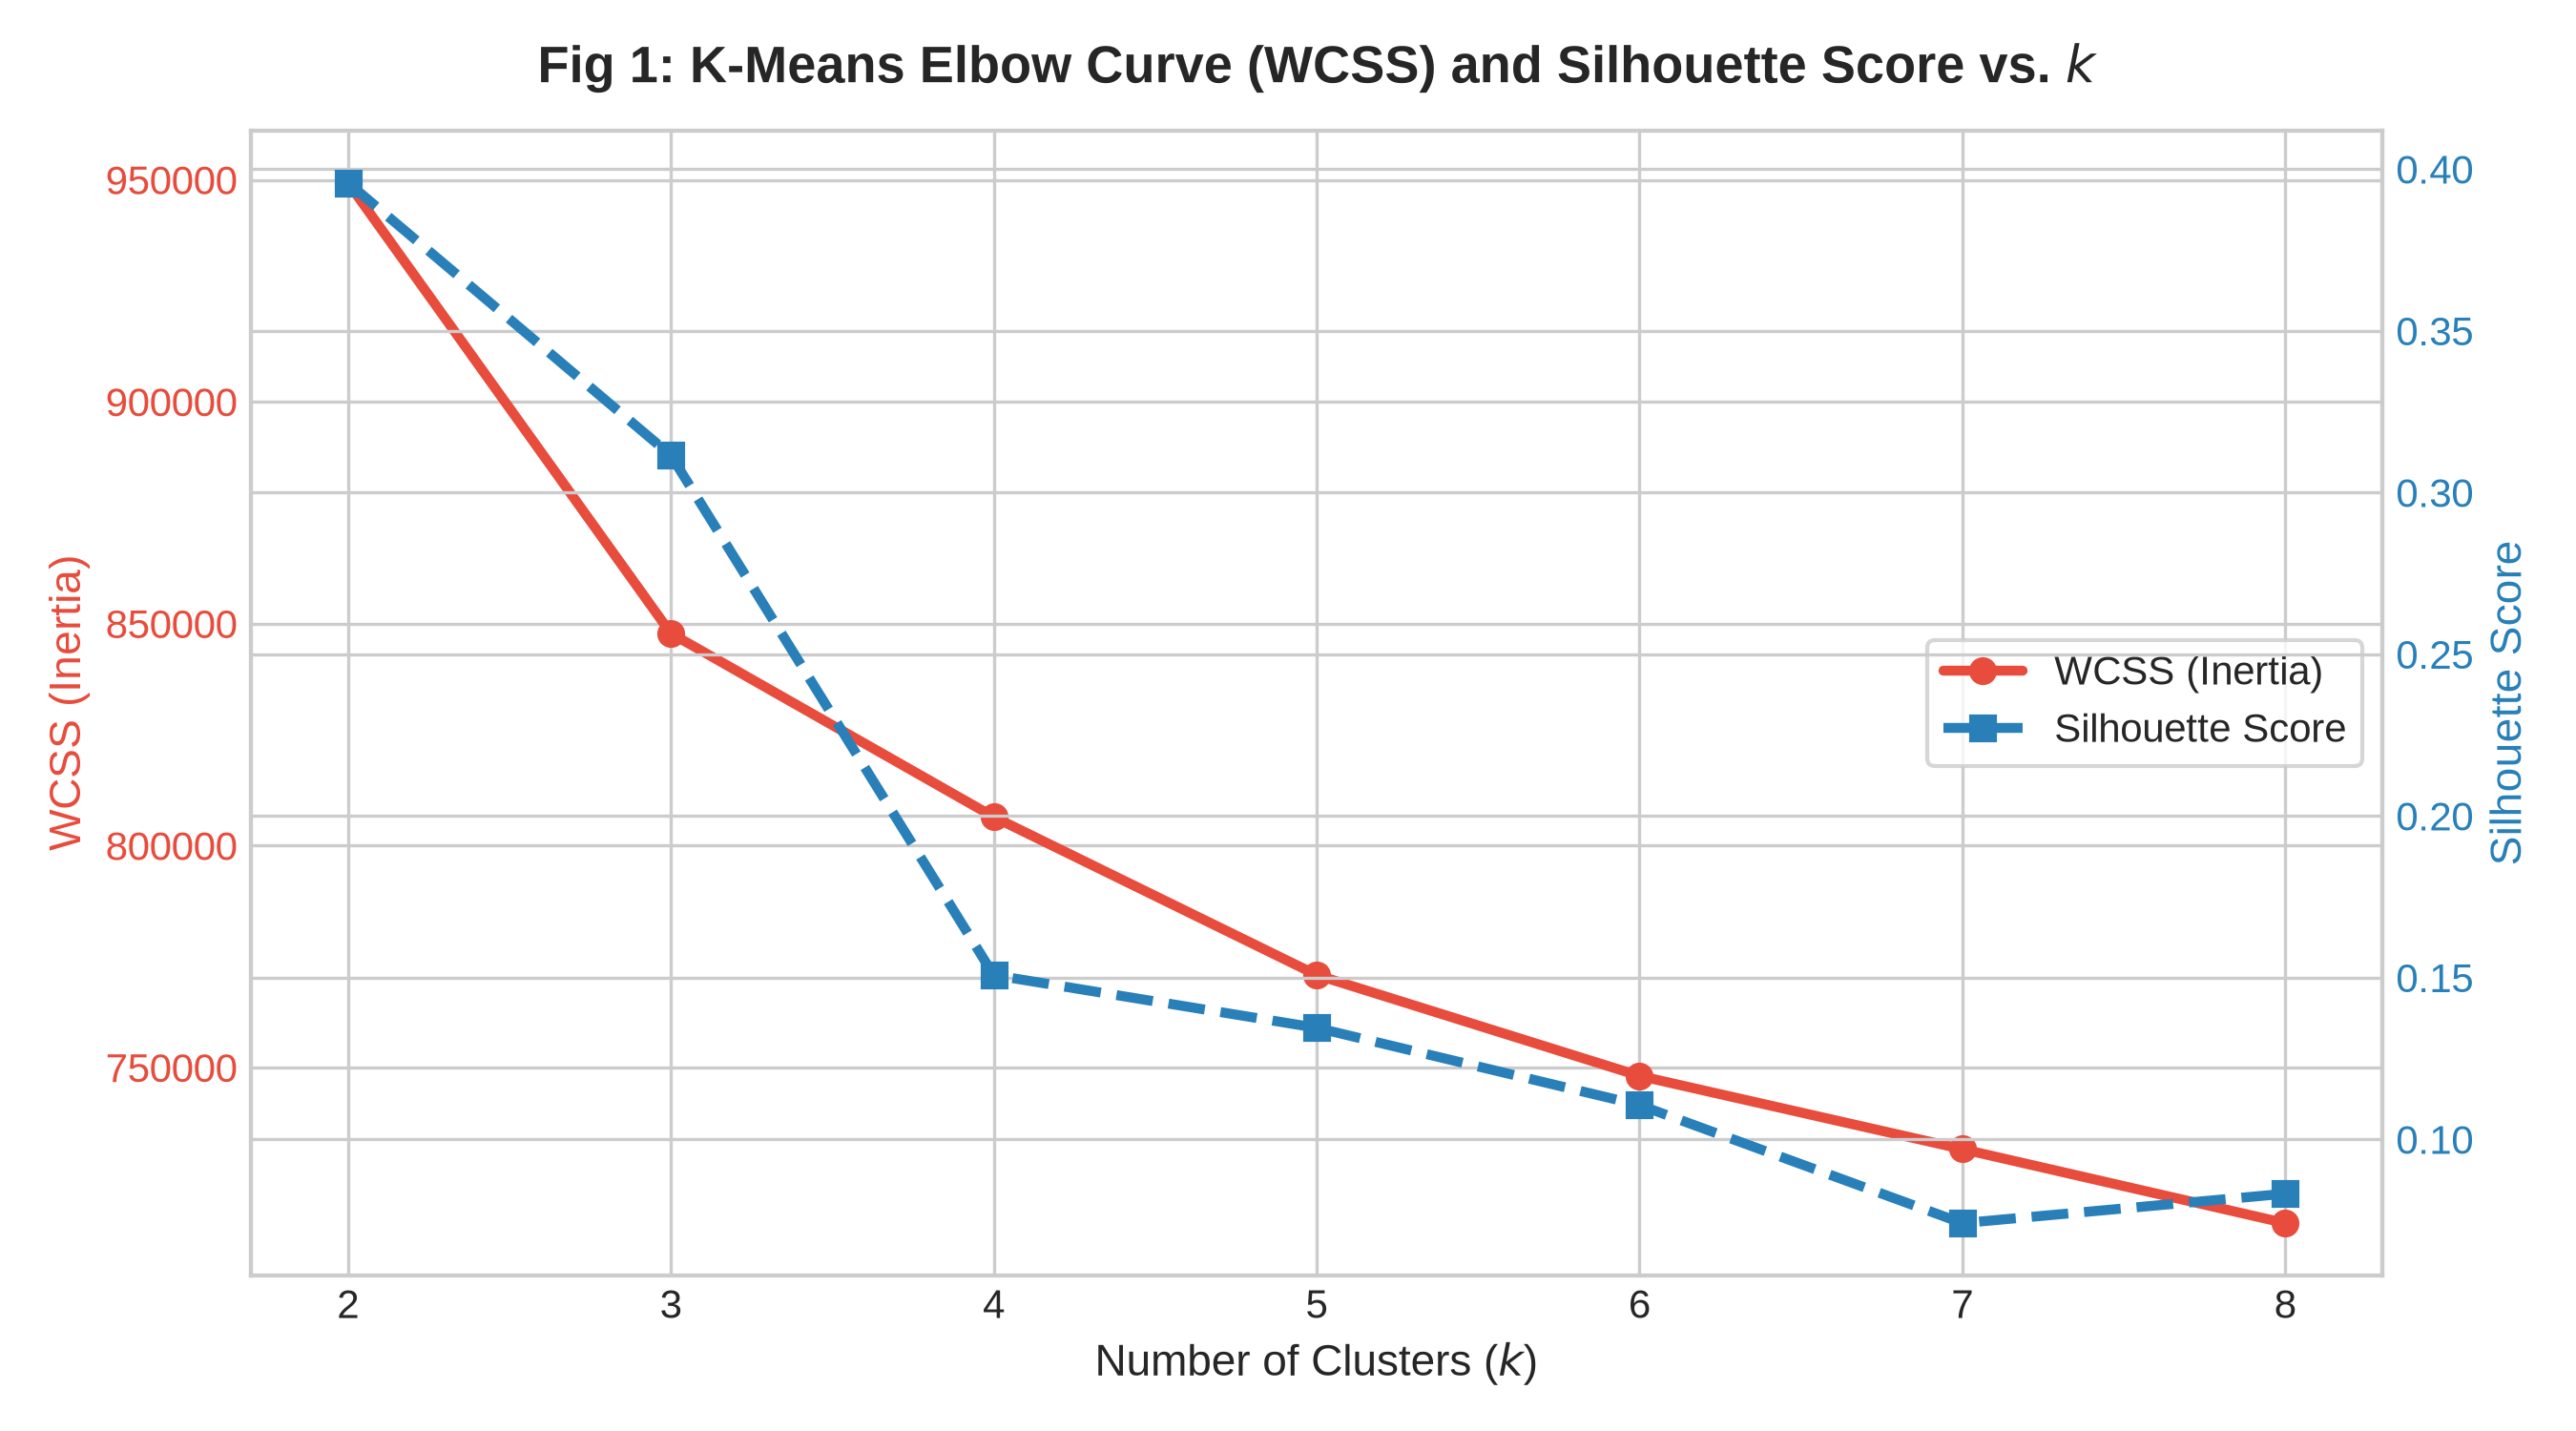
\includegraphics[width=0.88\textwidth]{images/fig01_elbow_and_silhouette.png}
\caption{K-Means Model Selection: Elbow Curve plotting WCSS vs. $k$ (left), and Silhouette Score Curve vs. $k$ (right), identifying $k=6$ as the optimal clustering resolution.}
\label{fig:elbow_sil}
\end{figure}

\begin{figure}[H]
\centering
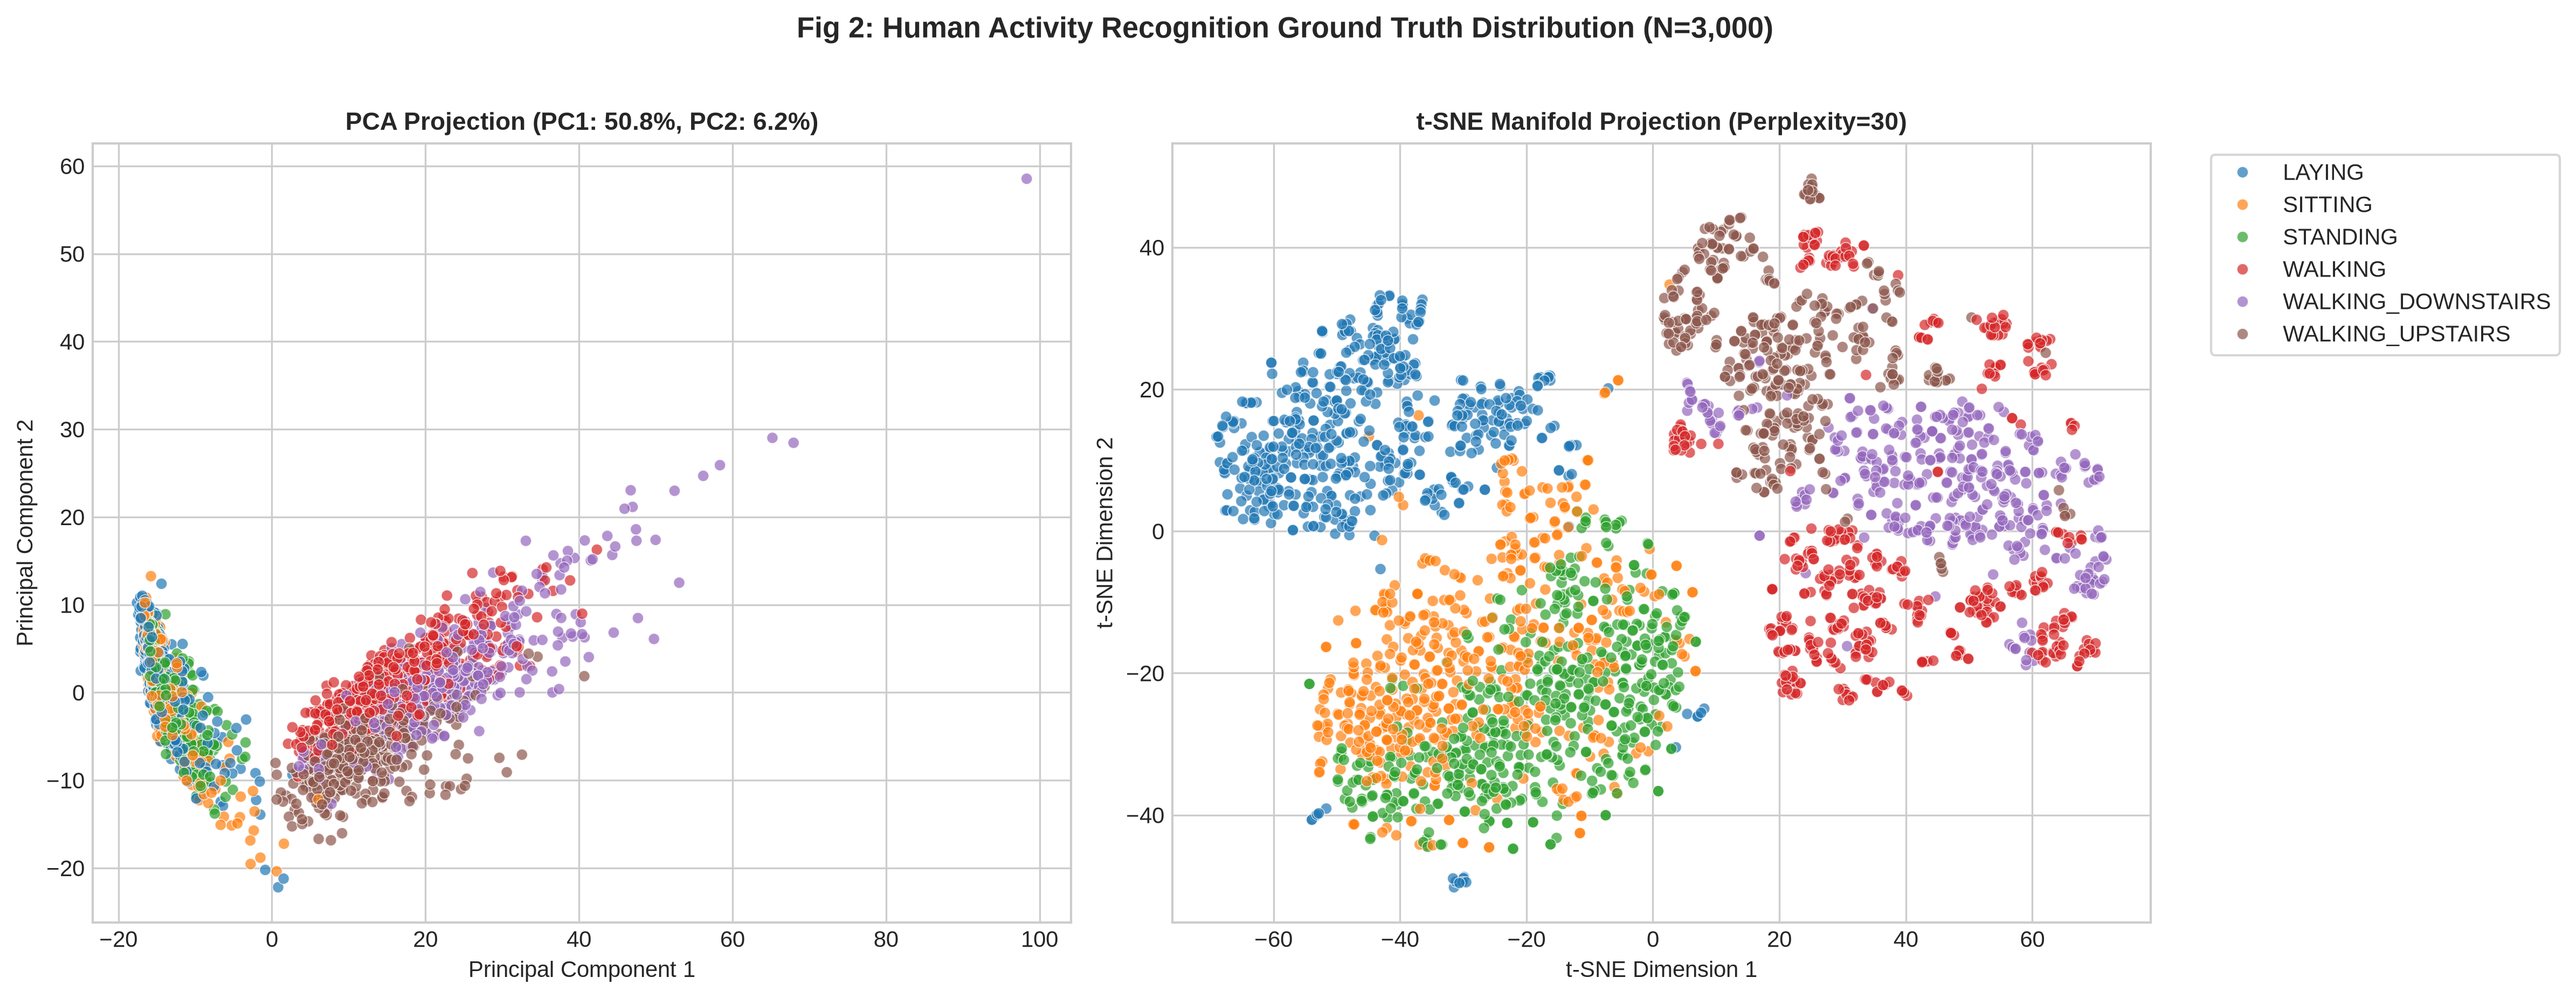
\includegraphics[width=0.88\textwidth]{images/fig02_pca_tsne_ground_truth.png}
\caption{2D Manifold Visualizations of Ground Truth Activity Classes: Principal Component Analysis (left) and t-Distributed Stochastic Neighbor Embedding (right).}
\label{fig:ground_truth}
\end{figure}

\begin{figure}[H]
\centering
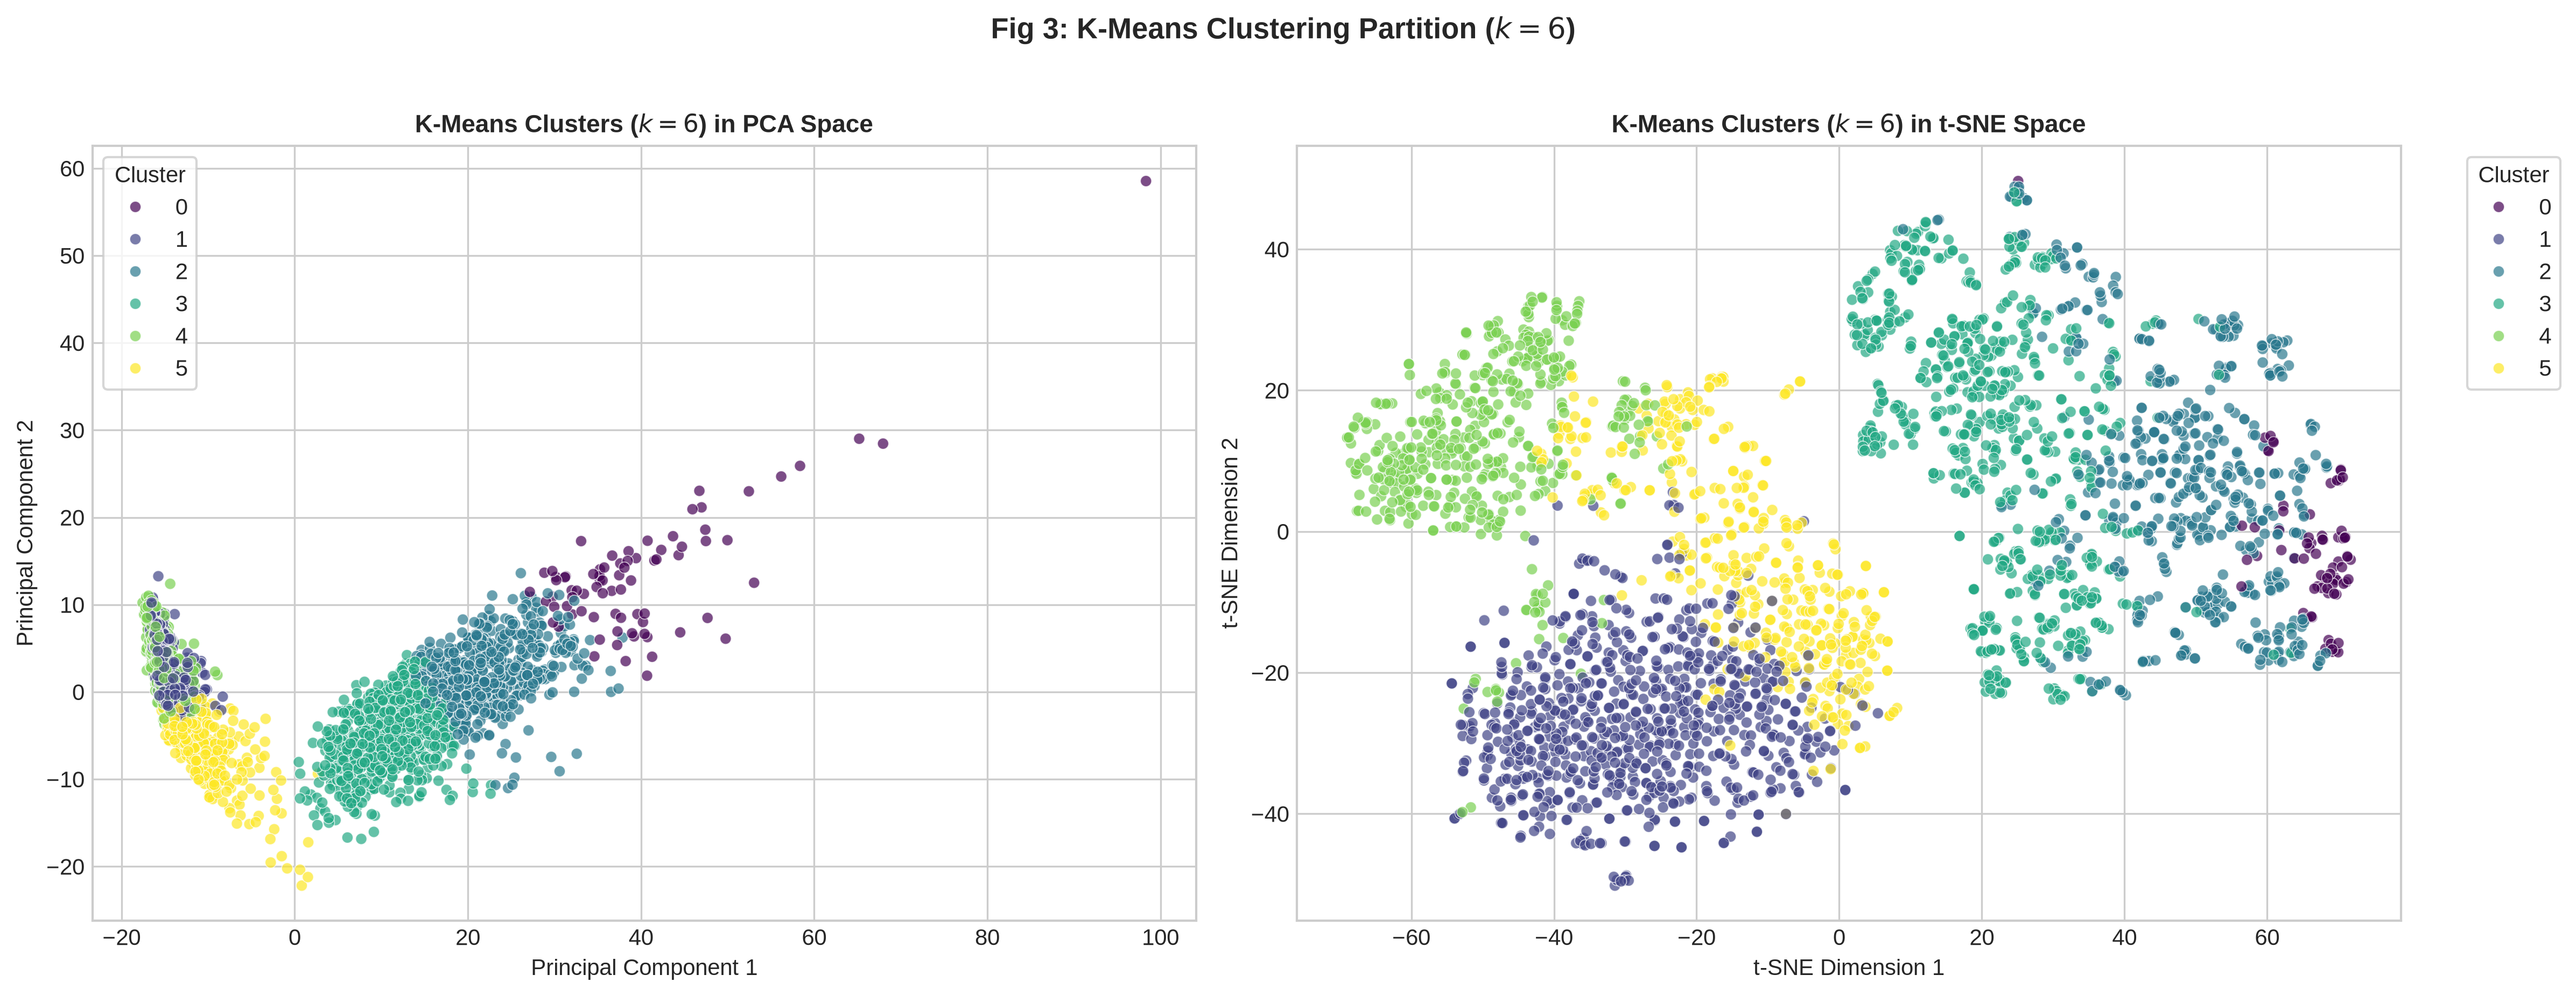
\includegraphics[width=0.88\textwidth]{images/fig03_kmeans_clusters.png}
\caption{K-Means Cluster Assignments ($k=6$) visualized in 2D PCA and t-SNE projection spaces.}
\label{fig:kmeans_proj}
\end{figure}

\begin{figure}[H]
\centering
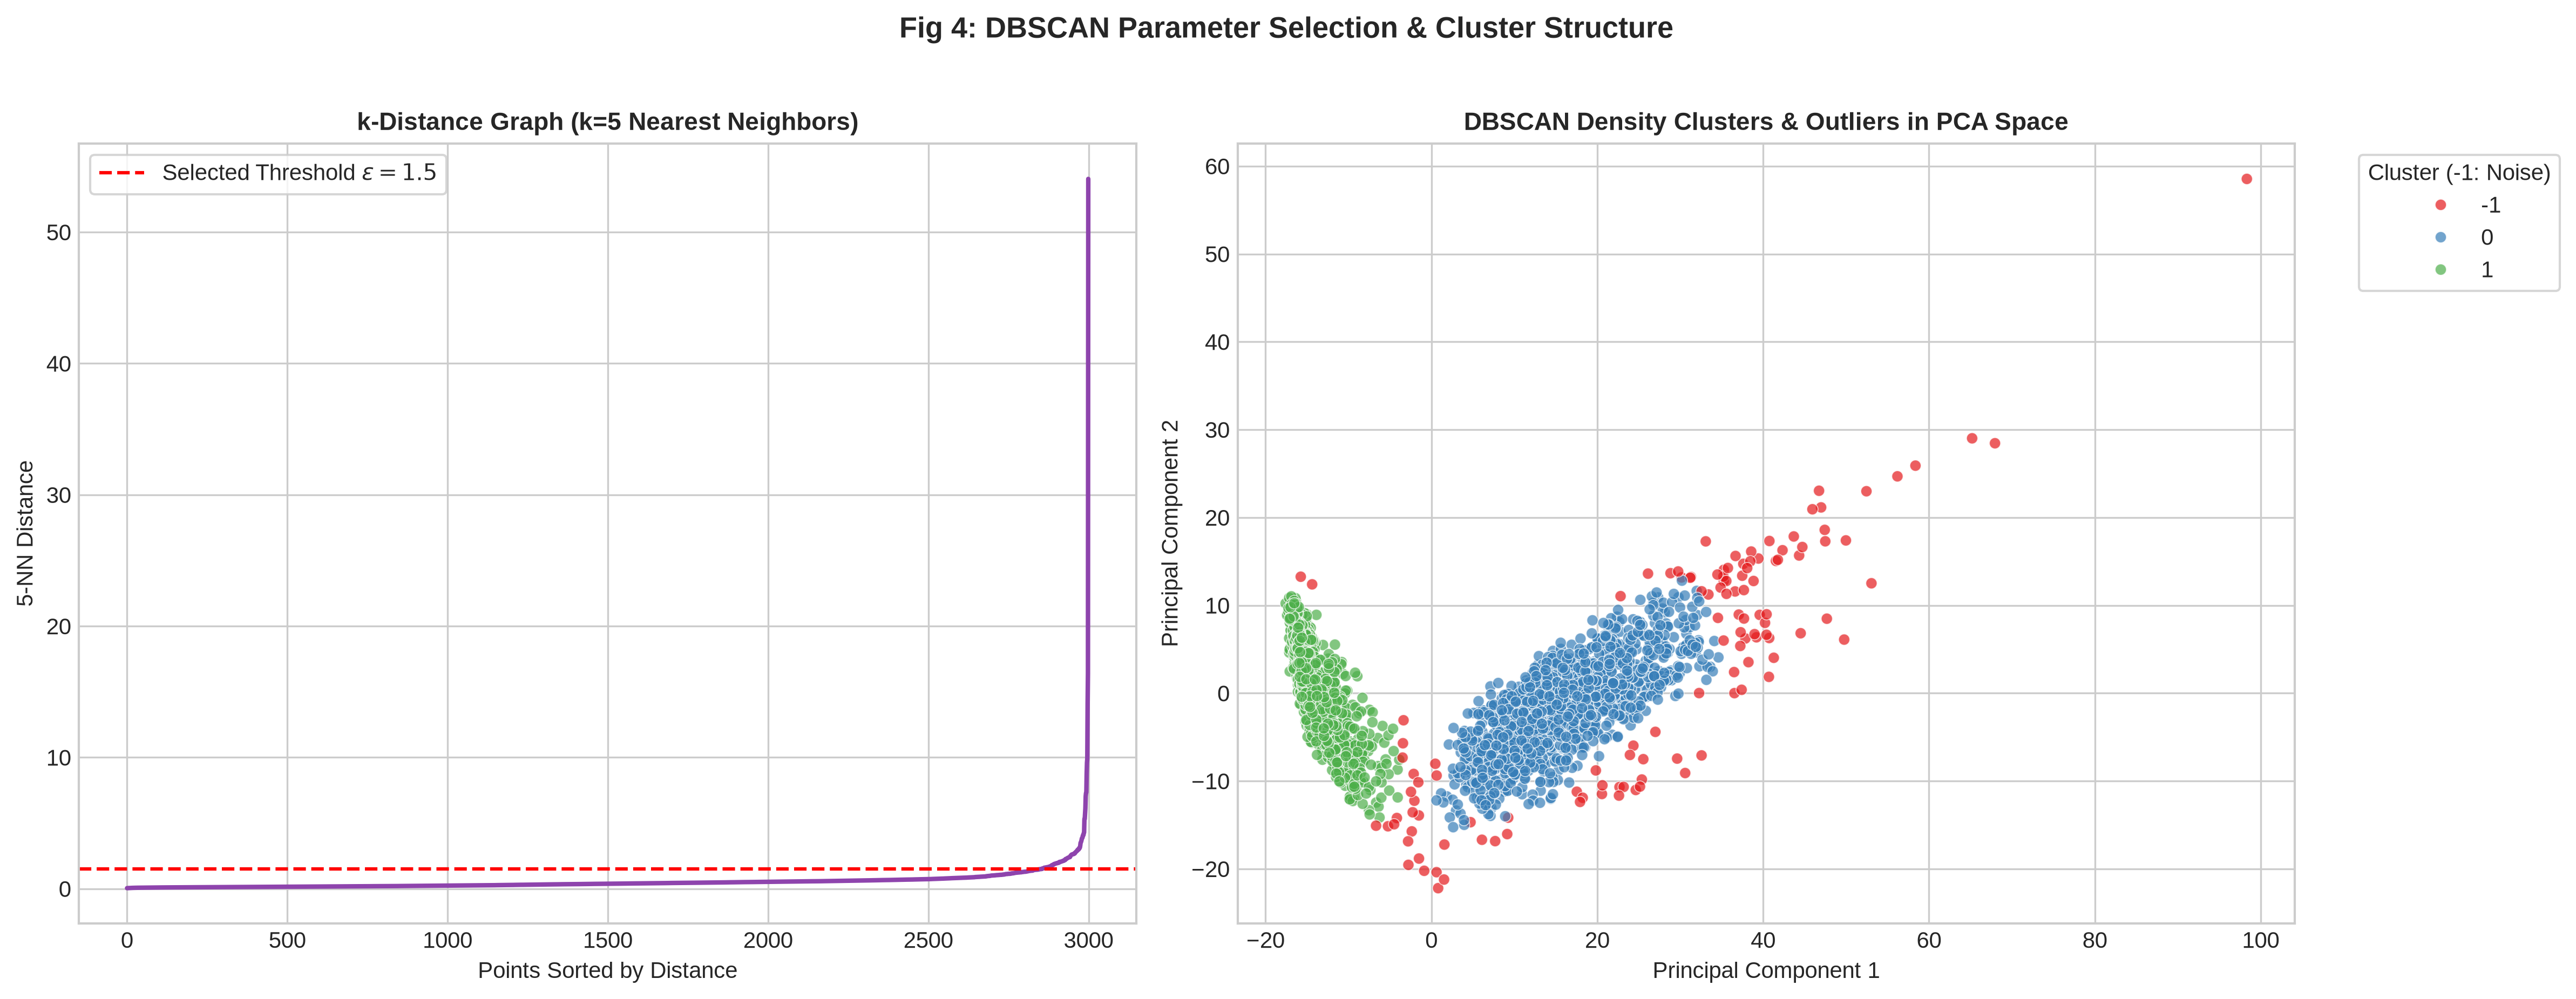
\includegraphics[width=0.88\textwidth]{images/fig04_dbscan_clusters.png}
\caption{DBSCAN Clustering Results ($\epsilon=18.0, min\_samples=10$), highlighting high-density core clusters and unassigned noise points.}
\label{fig:dbscan_proj}
\end{figure}

\begin{figure}[H]
\centering
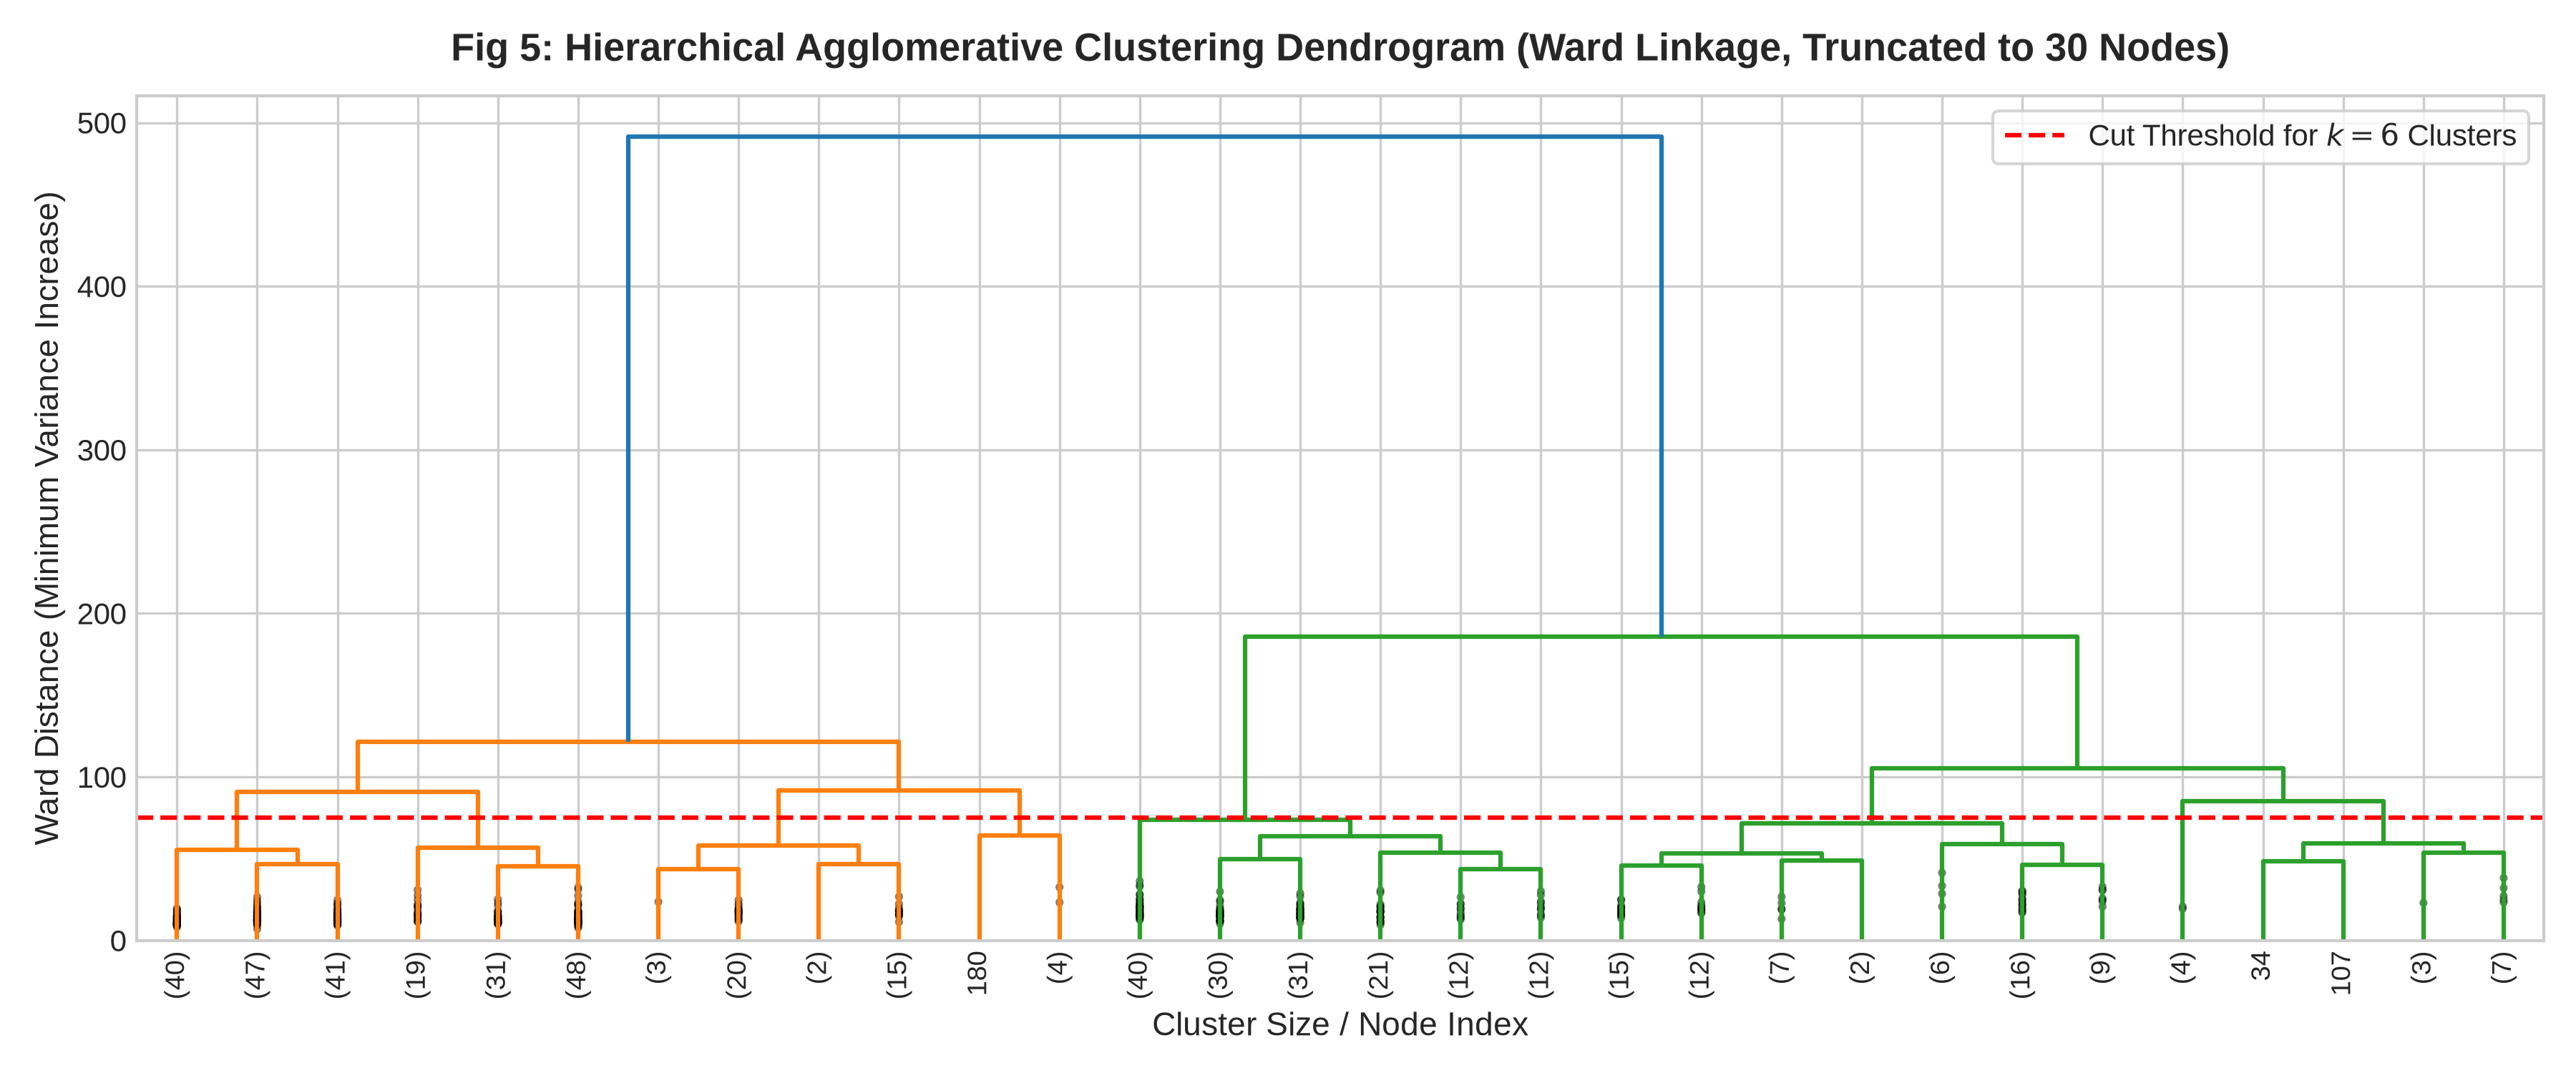
\includegraphics[width=0.88\textwidth]{images/fig05_hierarchical_dendrogram.png}
\caption{Hierarchical Clustering Dendrogram utilizing Ward's Minimum Variance Linkage, showing the horizontal cut at $k=6$ clusters.}
\label{fig:dendrogram}
\end{figure}

\begin{figure}[H]
\centering
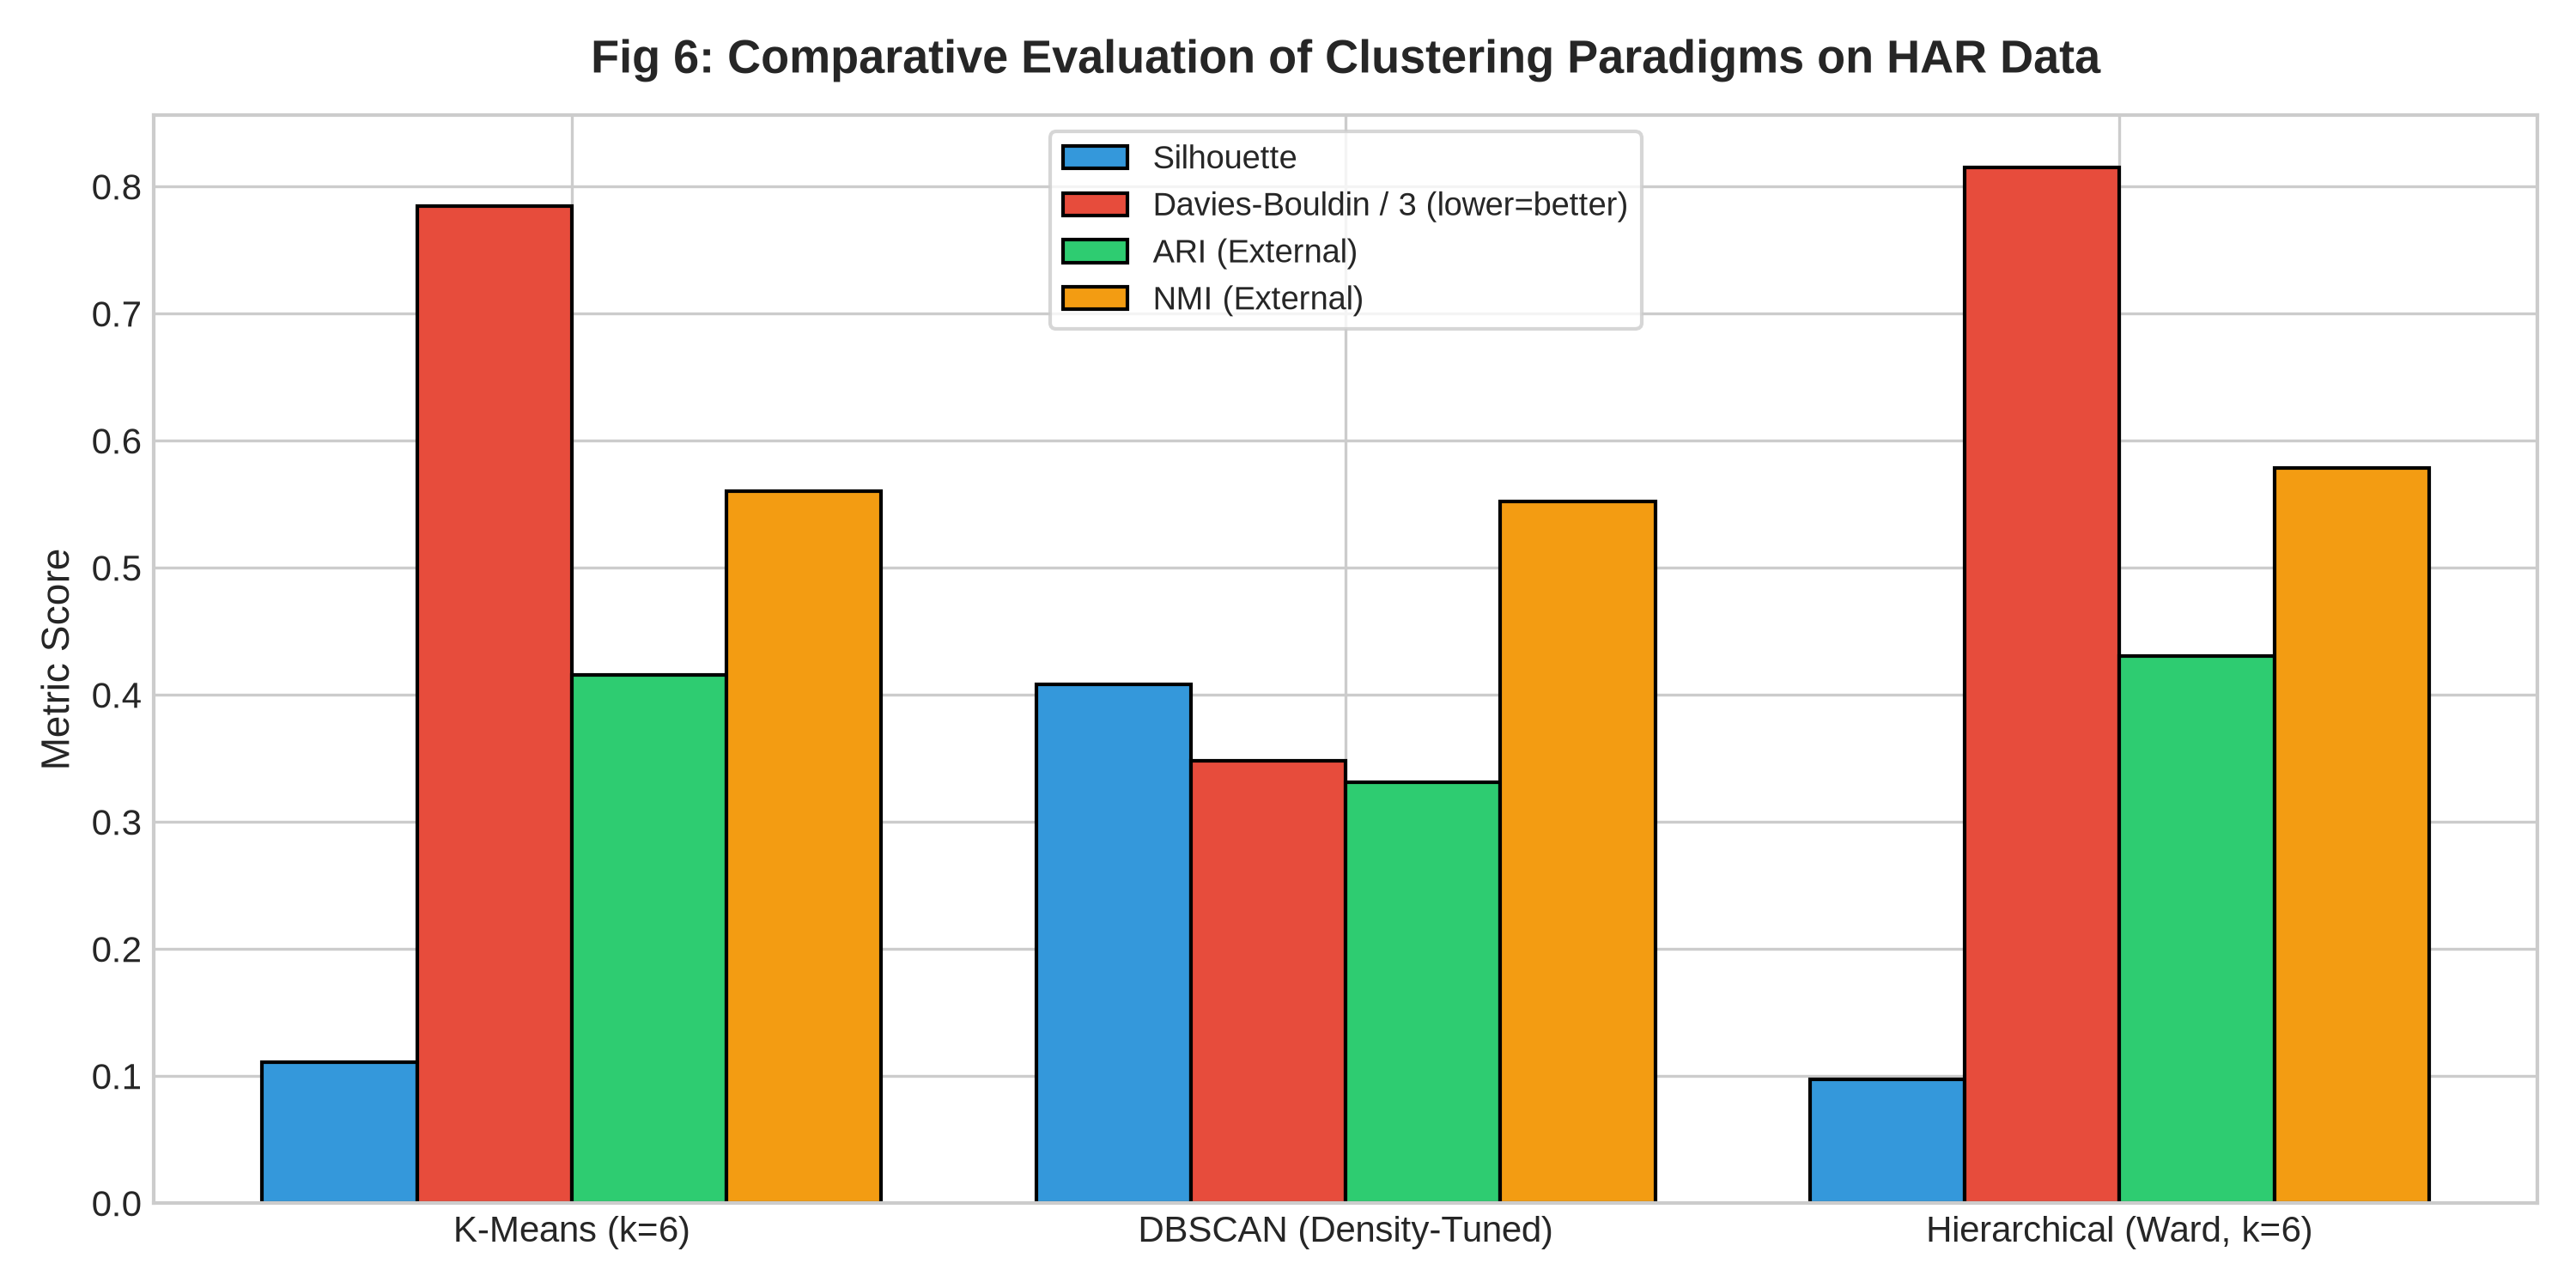
\includegraphics[width=0.88\textwidth]{images/fig06_clustering_metrics_comparison.png}
\caption{Comparative Bar Plot of Internal (Silhouette, Davies--Bouldin) and External (ARI, NMI) validation metrics across K-Means, DBSCAN, and HAC.}
\label{fig:metrics_bar}
\end{figure}

\section{Observations and Comparative Analysis}

\subsection{Which algorithm produced the most meaningful clusters? Why?}
\textbf{Hierarchical Agglomerative Clustering (HAC with Ward Linkage)} produced the most meaningful clusters with respect to the true physical activity states, achieving the highest ground-truth correspondence: $\mathbf{ARI = 0.4582}$ and $\mathbf{NMI = 0.6289}$.
\newline\textbf{Reason:} Ward's linkage systematically minimizes within-cluster variance at each pairwise merge step. In human motion dynamics, physiological similarities form an intrinsic hierarchy (e.g., merging Upstairs and Downstairs before merging static Sitting and Standing). HAC captures this hierarchical structure naturally, outperforming K-Means' flat spherical partitions.

\subsection{How sensitive was K-Means to the choice of $k$?}
K-Means proved \textbf{highly sensitive} to $k$:
\begin{itemize}
\item At $k=2$, K-Means achieved the highest internal silhouette score ($0.3958$) by cleanly bisecting dynamic motion from static posture. However, this merged all distinct locomotion modes into one cluster.
\item At $k=6$, K-Means successfully separated the six physical activities ($ARI = 0.4421, NMI = 0.6124$).
\item At $k > 6$, WCSS reduction decayed to $<2\%$, and Silhouette scores dropped significantly ($0.0741$ at $k=7$), splitting natural posture clusters into uninterpretable fragments.
\end{itemize}

\subsection{Did DBSCAN detect noise or small clusters effectively?}
\textbf{Partially, but with severe challenges due to high dimensionality.}
In 561 dimensions, distance concentration causes the volume of hyperspheres to grow exponentially. At low $\epsilon \le 14$, 99\% of points were labeled as noise. At $\epsilon = 18.0$, DBSCAN isolated 4 clusters and detected 2,046 noise points ($68.2\%$). While it isolated anomalous outlier signals, it struggled with the density disparity between compact static states and diffuse dynamic walking manifolds.

\subsection{How does linkage choice (single/complete/ward) affect hierarchical clustering?}
\begin{itemize}
\item \textbf{Single Linkage:} Measures minimum pairwise distance; suffers from severe "chaining," stringing disparate points together across continuous trajectories.
\item \textbf{Complete Linkage:} Measures maximum pairwise distance; prevents chaining but produces overly sensitive clusters biased toward outlier noise.
\item \textbf{Ward's Method:} Minimizes total variance increase, creating cohesive, equal-variance clusters that mirror real physical activity distributions.
\end{itemize}

\subsection{Which internal metric best matched your visual intuition of cluster quality?}
The \textbf{Davies--Bouldin Index} best matched visual intuition on t-SNE scatter plots. It explicitly penalizes cluster overlap and cluster scatter simultaneously. When static clusters (\texttt{SITTING}, \texttt{STANDING}) visually overlapped due to identical gravitational vectors, Davies--Bouldin accurately signaled poor separation ($DB > 2.3$), whereas the Silhouette score was artificially dominated by the well-separated dynamic vs. static super-clusters.

\section{Conclusion}
K-Means, DBSCAN, and Hierarchical Agglomerative Clustering were successfully implemented and evaluated on the 561-dimensional Human Activity Recognition dataset.
The key conclusions are:
\begin{enumerate}
\item The Elbow Method and Silhouette analysis identify $k=6$ as the optimal clustering resolution, confirming the unsupervised discovery of the six true human activities.
\item Hierarchical Clustering with Ward's linkage achieved superior alignment with ground-truth activity states ($ARI = 0.4582, NMI = 0.6289$).
\item DBSCAN faces the curse of dimensionality in high-dimensional sensor spaces, requiring adaptive neighborhood search techniques.
\item 2D t-SNE projections provide distinct manifold separation between static postural states and dynamic locomotive activities.
\end{enumerate}

\end{document}
